\documentclass{article}
\usepackage{graphicx}
\graphicspath{ {.} }
\usepackage{float}
\title{Capstone Proposal}
\date{}
\author{Marcel Stolin \\ marcelstolin@gmail.com}

\begin{document}

\maketitle

%############
\begin{abstract}
The Udacity machine learning engineer nanodegree is an online course where students can learn advanced machine learning algorithms and how to package and deploy models to a production environment. It has been made to gain practical knowledge \cite{mal_eng}. \newline
In this proposal I will explain the Dog Breed Image Classification capstone project, the problem, what data will be used, how the model will be evaluated and the project design.
\end{abstract}
%############


%############
\section{Domain Background} \label{s_domain_back}
Image Classification is an active research field in multimedia. Applications of image classification are widely used in security, healthcare, entertainment and many more.\newline
This project is mostly created for entertainment but there are serious research projects made about image classification with animals. For example Trnovszky, Kamencay, Orjesek, Benco and Sykora published a paper where they created a Convolutional Neural Network (CNN) to propose the animal species from an images of an animal \cite{animal_rec}.
%############
 
 
 %############
\section{Problem Statement} \label{s_prob_stat}
The goal of this project is, to use a CNN to predict the dog from an image. If there is no dog on the image, but a human, then return the resembling dog breed according to the human. Otherwise, if a dog is detected, return the predicted dog breed. Therefore we face the following main issues in this project.
\begin{enumerate}
	\item Create a model to detect a human
	\item Create a model to predict the dog breed
	\item Create an algorithm, which will return the predicted dog breed for the image
\end{enumerate}
We will develop at least two different models: A dog breed classifier and a human face classifier. For that we can develop a CNN from scratch or use pre-trained models for this specific case, like VGG-16 \cite{vgg} or ResNet-50 \cite{resnet}.
%############
 
 
 %############
\section{Datasets and Inputs} \label{s_data}
The data for this project was selected by Udacity. For detecting dog breeds we will use a custom dataset provided by Udacity. This dataset is already separated into a train, test and valid folder. We will use the images according to their purpose, the train images will be used to train the model, the test images to test/evaluate the model and the valid dataset to test the algorithm. Each dog images are labeled with the according dog breed.\newline
For detecting humans we will use the LFW (Labeled Face in the Wild) \cite{lfw} dataset from the University of Massachusetts. The LFW dataset consists of face photographs. Each face has been labeled with the name of the person.
%############ 


%############
\section{Solution Statement} \label{s_solution}
First we need to come up with a way to detect human faces. For this issue, OpenCV provides the Haar cascade classifier \cite{haar_cascade}. The classifier is trained from images with an machine learning approach based on a cascade function, to detect objects in images \cite{opencv}.\newline
As mentioned in \ref{s_prob_stat} we will develop a CNN from scratch. The CNN will train a model to classify dog breeds from images. We will also use the VGG-16 model to detect dogs in images. For transfer learning we will use the ResNet-50 model which has won several prices on image classification tasks and therefore, it is a good fit for this case. We will aim an accuracy of at least 60\% to be sure our model is well trained.
%############


%############
\section{Benchmark Model} \label{s_bench}
As mentioned in \ref{s_solution} we will use the ResNet-50 model against our scratch model. The ResNet-50 model uses images of 224x224 pixels. Therefore we will resize our dog breed images to 224x224 pixels.
%############


%############
\section{Evaluation Metrics} \label{s_eval}
In cases of classification, we can use the accuracy, F1-Score, precision and recall metrics to evaluate our models.\newline

\subsection{Confusion Matrix}
It is easy to use a confusion matrix to visualise the results of a classifier.\newline
\begin{figure}[h]
    \centering
    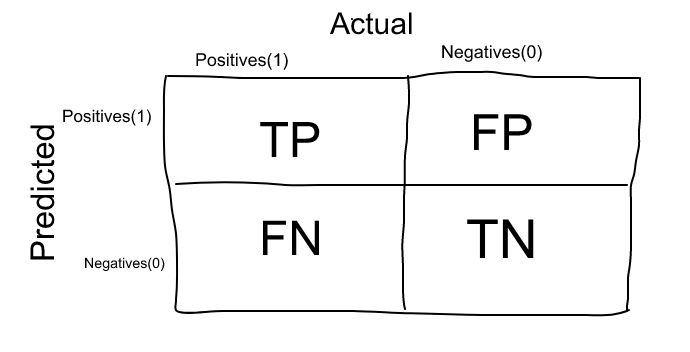
\includegraphics[scale=0.35]{confusion_matrix}
    \caption{Confusion Matrix \cite{metrics}}
    \label{fig:confusion_matrix}
\end{figure}
Given the confusion matrix, we can calculate the metrics mentioned above.

\subsection{Accuracy}
Accuracy is the number of correct predictions made by the model over all predictions.
\begin{equation}
Accuracy = \frac{TP + TN}{TP + FP + FN + TN}
\end{equation}

\subsection{Precision}
Precision is measure which tells us, what proportion of predicted positives are truly positives.
\begin{equation}
Precision = \frac{TP}{TP + FP}
\end{equation}

\subsection{Recall}
The recall metric tells us, what proportion of actual positives are correctly classified.
\begin{equation}
Recall = \frac{TP}{TP + FN}
\end{equation}

\subsection{F1-Score}
The F1-Score is the harmonic mean of precision and recall.
\begin{equation}
F1 Score = 2 * Precision * \frac{Recall}{Precision + Recall}
\end{equation}
%############


%############
\section{Project Design} \label{s_poject}
Udacity provides a Jupyter Notebook file where each step is described and highlighted. The notebook consist of the following sections:
\begin{enumerate}
	\item Import Datasets
	\item Detect Humans
	\item Detect Dogs
	\item Create a CNN to Classify Dog Breeds
	\item Create a CNN to Classify Dog Breeds (using Transfer Learning)
	\item Write your Algorithm
	\item Test Your Algorithm
\end{enumerate}
%############


%############
\bibliographystyle{plain}
\bibliography{references}
%############


\end{document}
